%%%%%%%%%%%%%%%%%%%%%%%%%%%%%%%%%%%%%%%%%%%%%%%%%%%%%%%%%%%%%%%%%%%%%%%%%%%%%%%
%% Descr:       Vorlage für Berichte der DHBW-Karlsruhe
%% Author:      Prof. Dr. Jürgen Vollmer, vollmer@dhbw-karlsruhe.de
%% Modified :	Nico Holzhäuser, TINF19B4
%% -*- coding: utf-8 -*-
%%%%%%%%%%%%%%%%%%%%%%%%%%%%%%%%%%%%%%%%%%%%%%%%%%%%%%%%%%%%%%%%%%%%%%%%%%%%%%%

\chapter{Clean Architecture}
\label{cleanArchitecture}
    Die Clean Architecture beschreibt eine bestimmte Methode, wie Software aufgebaut werden kann. Hierbei werden im weiteren 5 Schichten analysiert, welche im Projekt umgesetzt wurden.
    
    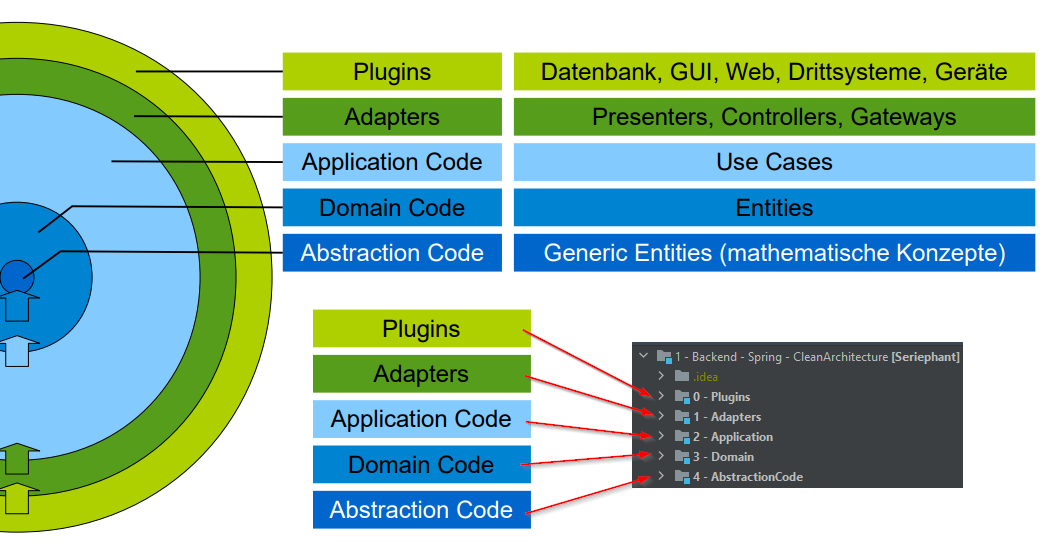
\includegraphics[width=0.95\textwidth]{zfiles/Bilder/schichten.png}

    \section{Schichtenarchitektur}
     Das Projekt soll sich an der Schichtenarchitektur orientieren. Hierbei sollen die einzelnen Module die einzelnen Schichten darstellen. Der Grund für die Benutzung einzelner Schichten ist die fachliche Unabhängigkeit der Anwendung von der sonstigen Infrastruktur. Dadurch können die einzelnen Teile leichter wiederverwendet, getestet und weiterentwickelt werden. Es ist auch leichter, einzelne Komponenten der Infrastruktur auszutauschen.
    
        \subsection{Abstraction - Schicht}
    	Diese Schicht stellt den Kern der Applikation dar. Hier werden Fundamente, oft durch die verwendete Programmiersprache geschaffen. Ein Beispiel hierfür ist die Implementierung des \hk{Strings} in Java, welche in der Spring Boot Anwendung verwendet wird.
    		\subsubsection{Implementierung im Projekt}
    		Diese Schicht wird durch Spring Boot,welches auf Java aufbaut, implementiert. 
    	
    	\subsection{Domain - Schicht}
    	In der Domain Schicht liegen die Business Objekte der Anwendung. Hier werden unternehmensweite Geschäftslogiken implementiert.
    		\subsubsection{Implementierung im Projekt}
    		In dieser Schicht liegen die Domänenobjekte, die Entities (\cref{1.entities}).
    	
    	\subsection{Application - Schicht}
    	In der Applikationsschicht liegen die Services, welche die Use-Cases implementieren.
    		\subsubsection{Implementierung im Projekt}
    		Die Use-Cases wurden in dieser Schicht implementiert, da sie über die Verantwortlichkeit einer einzelnen Entität hinausgehen. Diese Logiken und Prozesse wurden in sogenannte Services ausgelagert.
    	
    	\subsection{Adapters - Schicht}
    	In der Adapterschicht erfolgt die Umwandlung von Business-Objekten (interne Objekte) in Transferobjekten (externe Objekte).
    		\subsubsection{Implementierung im Projekt}
    		Hierzu werden Mapper verwendet, welche eine einfache Konvertierung von DTOs zu Entitäten und umgekehrt zulassen.
    		
    	\subsection{Plugins - Schicht}
    	In der Plugin-Schicht werden Frameworks verwendet. Diese unterstützen bestimmte Programmfunktionen, ohne diese selbst zu entwickeln und somit den selbt-geschriebenen Code zu minimieren.
    	    \subsubsection{Implementierung im Projekt}
    	    In diese Projekt sind mehrere Frameworks im Einsatz. \\
    	    \begin{itemize}
    	        \item Persistierungsframework --> Hibernate
    	        \item Debug-SQL-Console --> H2 Console
    	        \item API-Dokumentation \& Tests --> Swagger
    	    \end{itemize}

    \section{Frontend}
    Im Frontend mussten keine Prinzipien der Clean Architecture verwendet werden. Hier kommt React zum Einsatz, um die visuelle Darstellung der Use-Cases zu implementieren.